\chapter{领导的工作} % Introduction chapter suppressed from the table of contents

前面讲述了各种提高质量的最佳实践,如:测试驱动开发、结对编程等,可以让敏捷团队保证代码的质量;还介绍了如何利用数据做好冲刺复盘,找出根本原因,在下个迭代做好纠正措施。但是,要做到持续改善,管理层的支持是必要条件,管理层应如何支持敏捷团队的持续改进呢?\\

\hypertarget{ux6211ux4eecux5f88ux6ce8ux91cdux8d28ux91cfux4e0eux5ba2ux6237ux6ee1ux610fux5ea6}{%
\subsection{我们很注重质量与客户满意度}\label{ux6211ux4eecux5f88ux6ce8ux91cdux8d28ux91cfux4e0eux5ba2ux6237ux6ee1ux610fux5ea6}}

技术总监:我们公司是一家有着光荣历史的、上规模的国有企业,除了服务于各级政府单位,还为我们集团旗下的公司提供服务,这些公司在本行业领先全国,他们也都是国有企业,所以对质量要求挺高的。\\
我:请问有什么过程改进的案例吗?\\
技术总监:我们很重视客户满意度,首先要快速解决客户的问题,同时也会组织相关团队,从过程入手查原因,比如先从配置管理看是否有问题,然后从开发测试等一层一层去查看,最终找出原因并解决,定期给高层汇报,直到客户满意。\\
我:请举个实例。\\
技术总监:因为我们的客户要求非常严格,例如他们的发文都是正式的公文,不允许有任何差错。如果因为我们的系统导致发文出现问题,作为总监,我会亲自带领团队用上面的方法分析根因,而不仅仅靠下面的团队去解决。同时,我会把问题处理的进展汇报给总经理,让他知道我们在全力以赴,争取尽快解决问题。\\
我:你们高层关注哪些统计数据?\\
技术总监:我们很关注每位开发人员的代码生产率。我不知道有没有行业标准,我们的团队平均每人每天可以产出120行代码,估计离行业要求还是有差距。但是我们会朝行业标准方向逐步完善。\\
我:关于客户缺陷有什么统计?\\
技术总监:有的,我们会收集与分析(客户发现的)软件的缺陷数。\\
我:请问以往大概是什么水平?\\
技术总监:不太清楚,反正我们也关注。\\
我:你们公司不是希望从定性上升到定量管理吗?软件开发有个特点,缺陷发现得越晚返工越多,发现越早越容易解决(返工工时也小)。比如前面某北京公司,他们聘请了一位很有经验的质量总监,想改进公司的质量,但他不知道怎么去引起老板的关注,因他深知如果领导不了解质量有问题,后面就无法做任何改进。我建议他简单统计一下过去半年客户发现的缺陷数有多少,不过他们不一定有这些缺陷返工工作量的统计,但是可以在开始时先简单估算一下修复客户(发现的)缺陷耗费了公司多少成本,例如可以先利用美国的其他公司的历史统计数据,客户缺陷返工通常不会低于20人时,按这个便可以估算出因修复客户缺陷引起的质量成本,因缺陷耗费的工作量有多高。\\
技术总监:其实我们公司已经开始注重质量和质量成本,本来希望让财务去收集,但不知道如何入手。\\
我:单靠财务是无法收集到这些数值的,因为无法分辨哪些工作量是用于返工的,只有工程师才知道。所以必须由团队自己在迭代过程中收集,才能获得反映实际情况的数值。\\
技术总监:挺好,我们后面参考一下。\\
我:回到如何才能帮你们提升质量的问题。如果你们开始持续收集每个月的客户缺陷数,并且把它归一到缺陷密度,因为我们不能单收集缺陷数,项目有大有小,一个大项目的5个缺陷不能等同于小项目的5个缺陷,而缺陷密度就是缺陷数除以项目规模,所以缺陷密度相互之间就可以比较了。然后画出公司级的缺陷密度趋势图。例如我们之前有一家深圳国企客户,一直在收集并利用控制图监控投产通过率的上、下限,不但帮他们提高了质量的标杆或基线,还可以提供预警,例如在今年3月份,他们发现投产通过率特别低,他们不是用缺陷密度而是用投产成功率来计算的,因为他们的项目都是维护性的,有一些功能上的频繁更新,差不多两周要发版一次。从这个3月份的异常点,他们就做了一系列的根因分析,采取了应对的措施,这样水平就提高了,变成一个新的改善后的基线水平。你觉得这个思路可以用于你们公司的过程改进吗?\\
技术总监:对,你的建议挺好。我们后面会考虑引进你的方法。\\

\begin{description}
\item[]
\begin{description}
\tightlist
\item[]
= = =
\end{description}
\end{description}

正如首篇所说的,无论个人还是公司,所有改进(或创新)的前提是认识到现状与目标有差距。
从管理层关注的度量项可以反推公司会在哪方面有所改善,
如果管理层主要关注的是项目是否有延误,而不重视软件开发的质量,这将导致客户缺陷率不会有什么改善。

我们可以从以上故事了解到,高层都会说注重质量,但实际上不一定关注。如果要提升质量,首先要使用历史数据,画趋势图(控制图),知道自己当前的水平与范围(基线),利用控制图,识别异常点就可以帮公司预警,而不是应对客户投诉事件。应对投诉的根因分析属于救火。控制图(基线)也可以帮团队了解自己的质量在什么水平。有数据才有管理、改进。

\framebox{%
\begin{minipage}[t]{0.97\columnwidth}\raggedright
{问}:在传统 IT的
公司,无论是 Bug
率还是其他质量指标对业务的影响的相关性都不容易度量,只有重大事件才会让公司在客户面前失去信任,所以高层不会真正的重视质量。\\{答}:理解,但软件BUG的暴露越往后,返工的工作量就越高,而且是几何级数的增加(例如在单元测试或评审发现都可以1人时内解决;系统测试通常要花起码20人时,客户使用后才发现便更高)。但在很多IT公司,大部分缺陷都是在系统测试、甚至到验收测试才发现。如果能把软件缺陷的发现前移,把通过系统测试、验收测试发现的缺陷减半,便可以大量降低质量成本,提升开发生产率。所以我建议上面北京公司的质量总监利用缺陷数估算返工的工作量来引起老板重视。(而不是仅仅说降低缺陷率)\\{问}:有些业务客户可能不一定关注缺陷密度。举例:有些互联网公司关注系统的高可用性(按电信标准的99.99\%可用),因为高可用性会给业务上带来稳定的广告展现机会,也就是广告的库存。他们也关注上线后低异退率(如,上线后异退率:3/万,异退是各种复杂原因的异常退出),异退会对用户流失产生正相关的影响。\\{答}:系统的可用性,异退率等指标,也是可以连续收集到的(如,每天、每周),同样可以用上面深圳企业的方法,画控制图,预警过程有没有异常变动,如有异常便要启动根因分析,找到过程异常的根因,避免等到客户投诉才救火。\\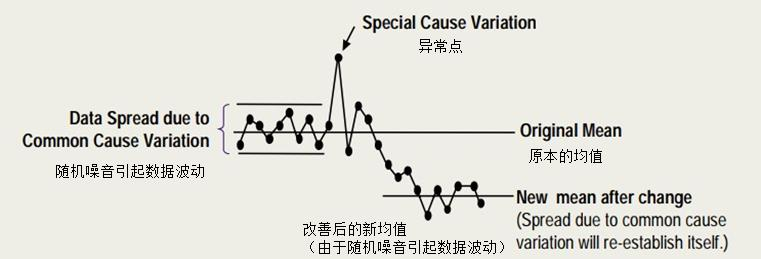
\includegraphics[width=6cm]{MGR_f11.jpg}\strut
\end{minipage}}

管理者应如何才能促进公司的持续提升?可以从下面的故事了解:\\

%\hypertarget{ux62c9ux5409ux592bux7ec8ux751fux53d7ux7528ux7684ux4e00ux4ef6ux4e8b}{%
%\section{拉吉夫终生受用的一件事}\label{ux62c9ux5409ux592bux7ec8ux751fux53d7ux7528ux7684ux4e00ux4ef6ux4e8b}}

\hypertarget{ux6211ux4eecux5f88ux6ce8ux91cdux8d28ux91cfux4e0eux5ba2ux6237ux6ee1ux610fux5ea6}{%
\subsection{拉吉夫终生受用的一件事}\label{ux6211ux4eecux5f88ux6ce8ux91cdux8d28ux91cfux4e0eux5ba2ux6237ux6ee1ux610fux5ea6}}


拉吉夫Rajiv Bajaj是印度著名的家族企业BAJIJ 的总裁。旗舰企业BAJAJ AUTO
是印度第二大的摩托车整车及配件生产商,印度市场销售三甲之一,年产销摩托车180万辆以上。他父亲巴贾吉
Raul BAJAJ 是企业创始人。

\begin{figure}
\centering
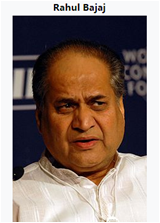
\includegraphics[width=2.60417in,height=\textheight]{Rajia1.png}
\caption{Raul BAJAJ,企业创始人}
\end{figure}

%\hypertarget{ux62c9ux5409ux592bux88abux9080ux8bf7ux5230ux4e00ux540dux6821ux6f14ux8bb2ux4ed6ux7528ux4e865ux5206ux949fux5206ux4eabux4e86ux4e00ux4f4dux65e5ux672cux987eux95eeux5bf9ux4ed6ux7ec8ux751fux53d7ux7528ux7684ux4e00ux4ef6ux4e8b}{%
%\subsection{拉吉夫被邀请到一名校演讲,他用了5分钟分享了一位日本顾问对他终生受用的一件事:}\label{ux62c9ux5409ux592bux88abux9080ux8bf7ux5230ux4e00ux540dux6821ux6f14ux8bb2ux4ed6ux7528ux4e865ux5206ux949fux5206ux4eabux4e86ux4e00ux4f4dux65e5ux672cux987eux95eeux5bf9ux4ed6ux7ec8ux751fux53d7ux7528ux7684ux4e00ux4ef6ux4e8b}}

\hypertarget{ux603bux7ed3}{%
\subsubsection{拉吉夫被邀请到一名校演讲,他用了5分钟分享了一位日本顾问对他终生受用的一件事:}\label{ux603bux7ed3}}


我第一次与一位日本顾问三口先生见面。

顾问:你在公司是做什么工作?What is your job?\\
我答:我就是这公司的总裁。\\
顾问:不是说你的职称,而是你的工作。\\
我答:开发不同样式的摩托车。\\
顾问:哦,你是做摩托车设计吗?

答:不是,我不是设计,我希望整个生产更有效率,减少浪费,例如,我们现在正尝试一个新概念
- 生产设计 (Design for Manufacturing)。

顾问:原来你是专管生产机器的?

答:不啊。

顾问:那你的工作是什么呢?

答:我的远景/目标是印度各地无论什么阶层,都购买我们各种各样的摩托车。

顾问说:哦,那你的工作是销售,与中间商签合作协议。

我有点生气地说:不,我不是销售。

顾问:听你的意思,既不是设计、生产和销售,你的工作是什么呢?

我无言以对。

顾问微笑地说:作为管理者,你的职责不是直接去做那些日常的工作,而是天天讲话、沟通。不是自己去工作,而是靠自己的影响力,来达到整个目的。

我有些了解了,谦虚地问:请告诉我,我的工作是什么?

顾问说:帮助整个公司改进就是你的工作,为你的公司员工提供一个环境,激发他们做好工作、提升公司,也给员工足够的权利把工作做好。

第二天,我们再次见面,山口先生又微笑着问我:\\
请告诉我你的工作。

我就满怀自信很高兴地说:我还记得你昨天的话,改进就是我的工作。

顾问就说:那么过了一天,你具体做了什么改进?

我又无法回答。

顾问接着说:印度人有一个通病,说得多,但是没有实际行动。

以上的故事深深让我领会到作为公司的最高领导,哪些是该抓的重点:应该依据公司面对的问题、困难:

\begin{enumerate}
\tightlist
\item
  定好一个明确的方向,而不是去处理各种杂事
\item
  需要协调好公司的总目标和每个部门的目标,避免方向不一致,导致混乱
\item
  每天思考做到了什么提升?
\item
  具体行动
\end{enumerate}

\begin{description}
\item[]
\begin{description}
\tightlist
\item[]
= = = = =
\end{description}
\end{description}

领导的最重要任务是制定、确定目标,(容易达到的目标不是好目标)
并提供相关培训、辅导,帮助团队提升;
而不是亲力亲为做,本来应该是团队负责的任务。

质量大师,如Dr
Juran,深深了解要提升公司,必须自来团队自身,而不是自上而下的家长式管理可以做到的。所以管理者必须从发号施令、指导下面团队的心态转换到我是老师/教练,辅导团队如何提升上来。

高层的管理风格会影响下面项目经理的心态与行为,也会影响在团队复盘时能否做好根因分析。下面是同一家公司,与技术总监下面某项目经理的交流:

\hypertarget{ux56e2ux961fux6839ux56e0ux5206ux6790}{%
\subsection{团队根因分析}\label{ux56e2ux961fux6839ux56e0ux5206ux6790}}

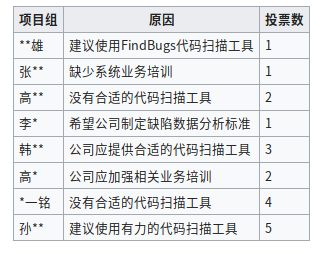
\includegraphics[width=6cm]{Screenshotfrom2022-12-2820-57-58.png}

我:从你们这根本原因分析记录,有没有看到你(雄)提出建议使用代码扫描工具后,其他7位团队成员中4位也提类似原因?\\
当团队一起围着开会时都会避免提出与众不同意见,所以当你邀请大家对提出的``原因''进行投票时,票数最多的也是你首先提出的扫描工具。

\framebox{%
\begin{minipage}[t]{0.97\columnwidth}\raggedright
我便用50年代群众压力实验问题
"请问右面ABC三条线那条线的长度最接近左面那条线的长度?" (Asch 1951)

跟项目经理解释:如果团队一起开会讨论,大家通常不会说自己的想法,难以集思广益。所以建议利用KJ方法(让每人自己写便利贴,贴在大白纸上,多轮``讨论''后,最终一起总结出主因),大家才能更好找到根因。\strut
\end{minipage}}

有没有发现你们提的原因其实都不是根因,都只是改正措施。
例如,缺乏工具,缺乏培训,缺乏标准等都是改进手段,不是根因。要不断地问为什么才可以找到根因。

如果没有找出根因前,直接寻找改正措施便不是对症下药,不能根治,问题可能很快又会重新浮现。

\hypertarget{ux603bux7ed3}{%
\subsubsection{总结}\label{ux603bux7ed3}}

若要敏捷团队能持续改进,为公司增值,\\
高层和经理都需要真正了解质量的重要性和现在团队的差距与不足,\\
并了解如何找出根因,避免问题重复发生,而不是仅仅应对问题(救火)。\\
要大家以数据说话,也不容易:

\hypertarget{ux4eceux5b9aux6027ux63d0ux5347ux5230ux5b9aux91cfux7ba1ux7406}{%
\subsection{从定性提升到定量管理}\label{ux4eceux5b9aux6027ux63d0ux5347ux5230ux5b9aux91cfux7ba1ux7406}}

有些研发总监有丰富的软件工程经验,但缺乏 业务的经验就不一定能把
运营的量化提升目标关联到研发团队的量化目标。例如:

\framebox{%
\begin{minipage}[t]{0.97\columnwidth}\raggedright
与北京某开发副总汇报:\\
我:公司的毛利要求从今年的32\%升到明年的35\%,请问你们有什么过程改进计划?\\
副总:我们最大的问题在需求与开发。\\
例如需求没有分析好各种场景 (Scenario, Use Case, User Story);
开发规范不足,也缺少复用; 依赖人工测试也是问题。\\
我:很好,但这些改进如何帮助公司提高毛利率\\
副总:这些改进点都能帮团队提升效率,毛利便自然会提升\\
我:我们有个好主意,可以帮你们容易地达成公司目标,毛利要求32\%升到35\%,有兴趣听吗?\\
副总:可以\\
然后我就跟他总结可以赋能团队分析每轮迭代的数据,并在下轮做改进,从而降低缺陷返工(质量成本),提升公司毛利:\\
现在大部分缺陷都是在系统测试阶段才被发现,据此估算缺陷返工成本占开发成本的30\%,如果能把缺陷提前在评审过程或单元测试阶段发现,就可以把返工成本占比降低到开发成本的15\%,也就能很轻松把毛利率提升到35\%,甚至更多。

现在都是由你们管理层分析,针对短板,制定总体改进措施。但每个小组的问题很可能不同,更应让团队针对哪些最困惑的不足,做改进。

软件开发,与工厂生产不同,过程数据都要依赖开发人员自己统计收集,但要他们有动力不断收集数据,必须要有定期反馈,让他们知道数据对他们的用途。

如果你们高层收基并分析数据,然后改进,前后最快也得要两三个月;但如果让他们整个团队在每一次迭代回顾时分析数据,他们就有动力在下一轮迭代继续收集数据,因为他们知道数据都会在回顾时讨论;也因为他们要参与讨论决定改进措施,他们才有动力,在下一个迭代执行改进措施。

\begin{description}
\item[]
\begin{description}
\tightlist
\item[]
。 。 。
\end{description}
\end{description}

45分钟的交流结束后,副总在总结时提到他本来的关注点:
``你们关于差距分析的发现很正确,尤其是需求场景分析,后续希望请你们帮我们加强需求场景的培训。''\strut
\end{minipage}}

因为副总的软件工程经验很丰富,他非常理解如果需求、开发、测试等做得不好,都会影响项目质量。很多有开发经验的领导都会集中精力把事情做好,例如:需求、开发,但这反而影响他们难以抽身出来,从总体业务的视角,利用数据,做好管理。

有效过程改进必须先从团队开始,而不是靠从上而下的指挥;
要从定性管理思维模式提升到定量管理, 必须是整个公司从上而下的范式转移
(paradigm shift) , 才能给敏捷团队持续改善的土壤,\\
或者通俗来讲 - 公司文化。




